%!TEX root=demo-paper.tex

\section{System architecure}
\label{sec:system_architecture}

In this section, we present the architecture of \SeeDB\ starting with an
overview, followed by a detailed discussion of the various modules in \SeeDB.

\subsection{{\large \SeeDB} architecture overview}
\label{subsec:overview}

Our prototype of \SeeDB\ is designed as a layer on top of a traditional
relational database system.
While optimization opportunities are restricted by virtue of being a layer outside the
database, our design permits \SeeDB\ to be used in conjunction with a variety of
existing database systems. 
\SeeDB\ is comprised of two main parts: the \SeeDB\
frontend and the \SeeDB\ backend. The frontend is a ``thin client'' that
is only used to issue queries to \SeeDB\ and view results. The backend, in
contrast, performs all the computation required to generate and select views
to be recommended. Figure \ref{fig:sys-arch}
depicts the architecture of our system.

\begin{figure}[htb]
\vspace{-10pt}
\centerline{
\hbox{\resizebox{9cm}{!}{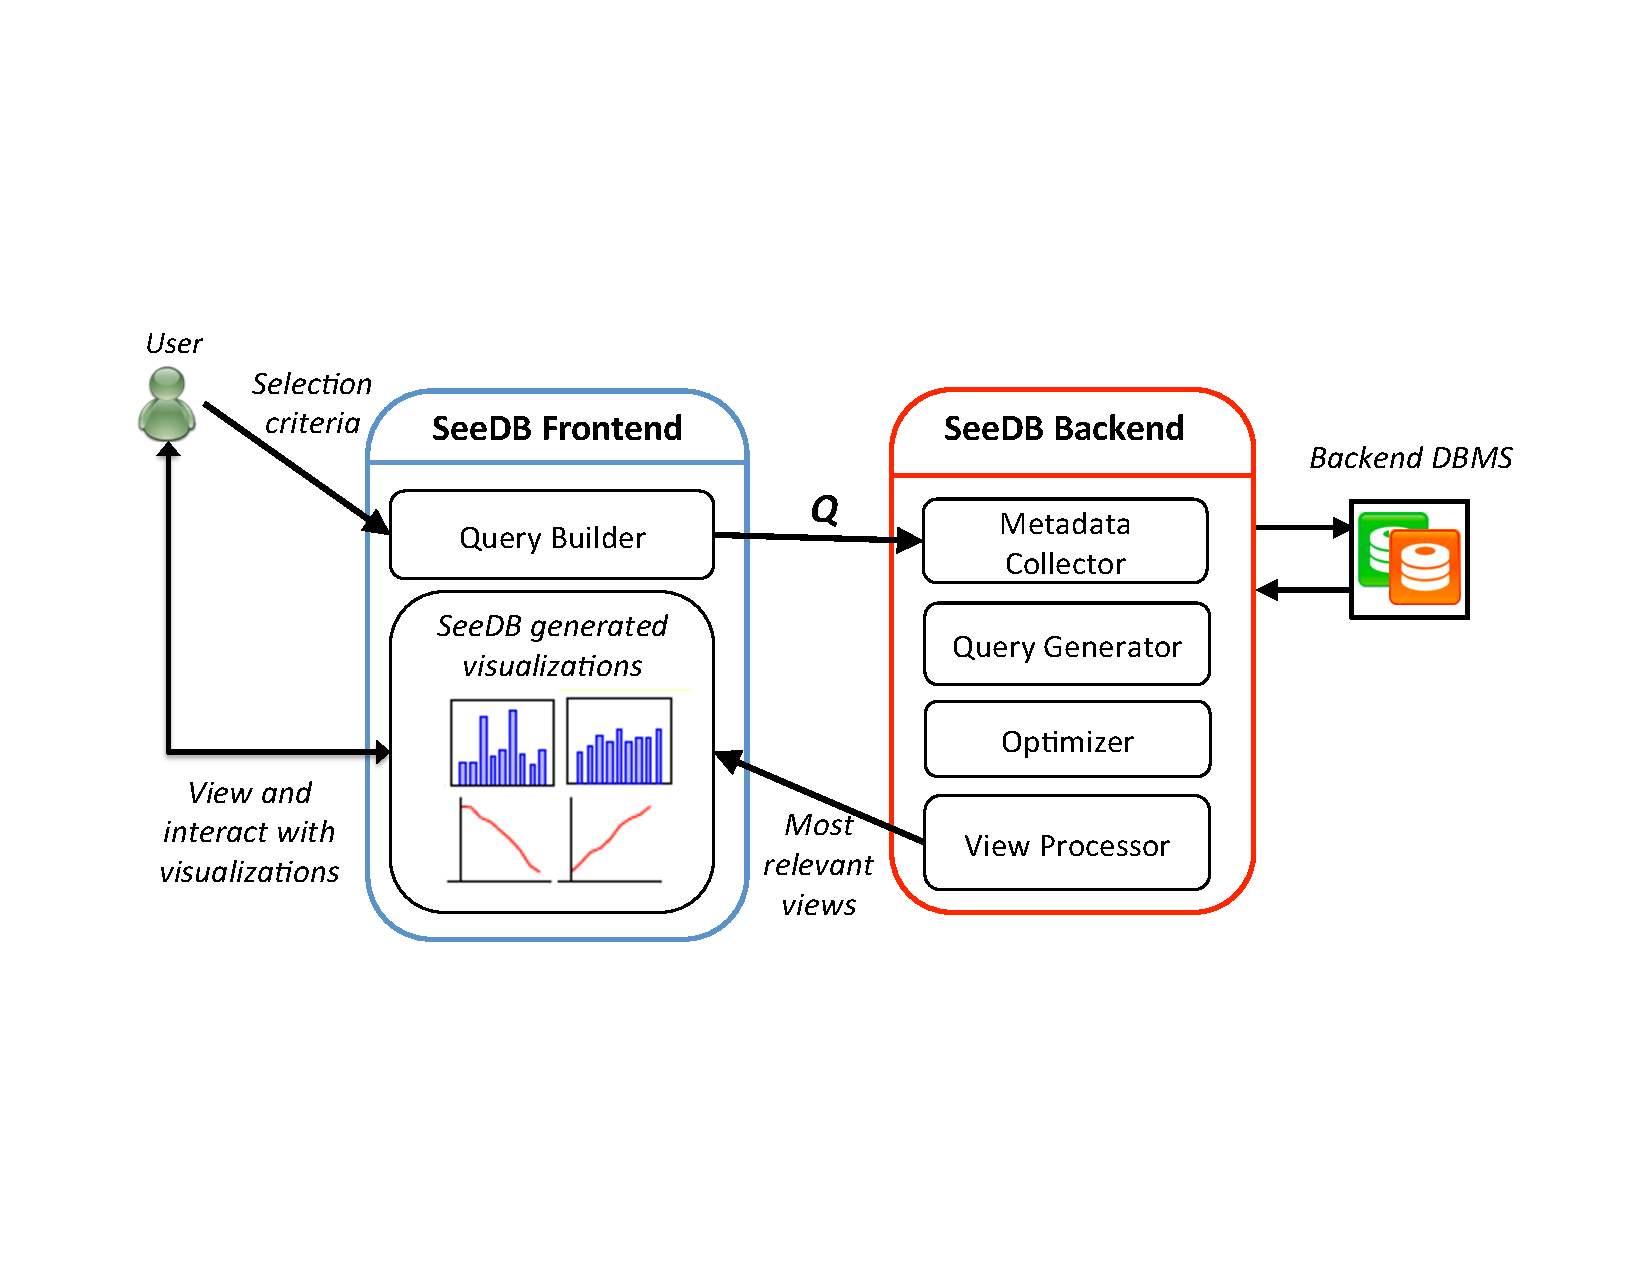
\includegraphics[trim=10mm 50mm 10mm 50mm,
clip=true]{Images/seedb-architecture.pdf}}}}
\caption{SeeDB Architecture}
\label{fig:sys-arch}
\vspace{-10pt}
\end{figure} 

An analyst uses the frontend to issue queries to \SeeDB. We provide three
mechanisms for the analyst to issue queries, of which only the intuitive
query-builder tool mechanism is depicted in Figure~\ref{fig:sys-arch} 
(we discuss query input further in Section \ref{subsec:seedb_frontend}).
Once the analyst issues a query via the frontend, the backend
takes over.
First, the Metadata Collector module queries metadata tables (a combination of
database-provided and \SeeDB\ specific tables) for information such as table
sizes, column types, data distribution, and table access patterns.
The resulting metadata along with the analyst's query is then passed to the
Query Generator module. The purpose of the Query Generator is two-fold:
first, it uses the metadata collected to prune the space of
candidate views to only retain the most promising ones; and second, it generates target and
comparison views for each view that has not been pruned.
The SQL queries corresponding to the target and comparison views are then passed
to the Optimizer module. We refer to these queries collectively as {\it view
queries}.
Next, the Optimizer module is responsible for determining the best way to combine
view queries intelligently so that the total execution time is minimized. 
(We discuss the optimizations performed by the Query Generator and
Optimizer modules further in Section \ref{subsec:seedb_backend}.) Once the
Optimizer module has generated the optimized queries, \SeeDB\ issues the
queries to the underlying database system for execution. The results returned by
the DBMS are then processed by the View Processor module. This module processes
results of the optimized queries in a streaming fashion and produces results for
each individual view. The results of individual views are then normalized as discussed
in Section~\ref{sec:problem_statement} and the utility of each view is computed.
Finally \SeeDB\ selects the top $k$ views with the highest utility and returns them to the
\SeeDB\ frontend. The \SeeDB\ frontend generates visualizations for each
view and displays them.

We now discuss the major \SeeDB\ modules in detail.

\subsection{SeeDB Frontend}
\label{subsec:seedb_frontend}

The \SeeDB\ frontend, designed as a thin client, performs two main functions: it
allows the analyst to issue a query to \SeeDB, 
and it visualizes the results (views) produced by the \SeeDB\
backend.
To provide the analyst maximum flexibility in issuing queries, \SeeDB\
provides the analyst with three
mechanisms for specifying an input query: 
(a) directly filling in SQL into a text box, 
(b) using a query builder tool that allows analysts
unfamiliar with SQL to formulate queries through a form-based interface, and (c)
using pre-defined query templates which encode commonly performed operations,
e.g., selecting outliers in a particular column. We find that pre-defined query
templates are particularly useful since analysts are often interested in
anomalous data points.

Once the analyst issues a query via the \SeeDB\ frontend, the \SeeDB\ backend
evaluates various views and then 
computes and delivers the most interesting ones (based on utility) back to the frontend.
For each view delivered by the backend, the \SeeDB\ frontend determines the visualization
for the view depending on parameters such as the data
type (e.g. ordinal, numeric), number of distinct values, and semantics (e.g.
geography vs. time series).
The resulting set of visualizations is displayed to the analyst who can then
easily examine these ``most interesting'' views at a glance, explore specific views in
detail by hovering and clicking on various portions of the view, 
and study metadata for each view (e.g. size of result, sample data, value with
maximum change and other statistics). 
The analyst can also slice-and-dice views further by performing drill-downs on
specific attributes in the view. 
Figure~\ref{} \agp{missing..} shows a screenshot of the \SeeDB\ frontend in action.
%This action automatically
%modifies the selection query and displays views for the subset of data
% selected. The user can of course revert back to the original views and continue exploring the data.

\subsection{SeeDB Backend}
\label{subsec:seedb_backend}

The \SeeDB\ backend is responsible for all the computations for 
generating and selecting views. 
\agp{next line can be deleted if needing space, repetitive.}
As shown in Figure~\ref{fig:sys-arch}, the \SeeDB\ backend is composed of four
modules that are respectively responsible for collecting metadata (Metadata Collector), pruning
the view space and generating view queries (Query Generator), optimizing view
queries (Optimizer), and processing query results to identify the top-$k$
interesting views (View Processor). 
To achieve its goal of finding the most
interesting views accurately and efficiently, the \SeeDB\ backend must not only accurately
estimate the accuracy of a large number of views but also design ways in which
the total processing time will be minimized.
We first describe the basic \SeeDB\ backend framework and then briefly discuss our optimizations.

% One of the chief challenges in \SeeDB\ is producing the most interesting views
% of the query result in the least possible time. For achieve the above
% performance goal, \SeeDB\ must perform optimizations at two stages: first, using
% prior knowledge such as statistics to prune out uninteresting views without examining table data; and second, minimizing the
% execution time for queries that are issued to the database. 

\subsubsection{Basic Framework}
\label{subsubsec:basic_framework}

Given a user query $Q$, the basic approach would be to compute all
possible views obtained by adding a single aggregate and a single group-by
clause to $Q$ \agp{two column?}. 
The target and comparison views corresponding to each view are then
computed and each view query is executed independently on the DBMS. The query
results for each view are normalized to obtain the target and comparison view
probability distributions, and the utility of a given view is computed as the
distance between these two distributions (Section \ref{sec:problem_statement}).
Finally, the top-$k$ views with the largest utility are chosen to be displayed. 

The basic approach is clearly inefficient
since it examines every single possible view 
and executes each view query independently;
we next discuss how our optimizations fix some of these problems.

\subsubsection{View Space Pruning}
\label{subsubsec:view_space_pruning}

In practice, most views for any query $Q$ have low utility since the target view
distribution is very similar to the comparison view distribution. 
\SeeDB\ uses this property to aggressively prune 
view queries that are unlikely to have high utility. 
This pruning is based on metadata about the table including data
distributions and access patterns.
We leverage table metadata in several ways, some of which are listed below:
\begin{denselist}
\item {\it Variance-based pruning}: Dimension attributes with low variance are
likely to produce views having low utility (e.g. consider the extreme case where
an attribute only takes a single value); \SeeDB\ therefore prunes views
containing grouping attributes with low variance.
\item {\it Correlated attributes}: If two dimension attributes $a_i$ and $a_j$ have
a high degree of correlation (e.g. full name of airport and abbreviated name of
airport), the views generated by grouping the table on $a_i$ and $a_j$ will be
very similar (and have almost equal utility). We can therefore generate and
evaluate a single view representing both $a_i$ and $a_j$. \SeeDB\ clusters
dimension and measure attributes based on correlation and evaluates a single representative view per
cluster.
\item {\it Access frequency-based pruning}: In tables with a large number of
attributes, only a small subset of attributes are relevant to the analyst and
are therefore frequently accessed for data analysis. \SeeDB\ tracks access patterns
for each table to identify the most frequently accessed columns and combinations of
columns. While creating views, \SeeDB\ uses this information to prune attributes
that are rarely accessed and are thus likely to be unimportant.
\end{denselist}

\subsubsection{View Query Optimizations}
\label{subsubsec:optimizations}

The second set of optimizations used by \SeeDB\ minimizes the execution time for
view queries that haven't been pruned using the techniques described above.
Since view queries tend to be very similar in structure (they differ in the aggregation
attribute, grouping attribute or subset of data queried), \SeeDB\ uses multiple
techniques to intelligently combine view queries.
The ultimate goal is to minimize scans of the underlying dataset by sharing as
many table scans as possible. Our optimization strategies include:

\begin{denselist}
  \item {\it Combine target and comparison view query}: Since the target view
  and comparison views only differ in the subset of data that the query is
  executed on, we can easily rewrite these two view queries as one.
  This simple optimization halves the time required to compute the results for
  a single view.
  \item {\it Combine Multiple Aggregates}: A large number of view
  queries have the same group-by attribute but different aggregation attributes.
  Therefore, \SeeDB\ combines all view queries with the same group-by attribute
  into a single query. This rewriting provides a speed up linear in the
  number of aggregate attributes.
  \item {\it Combine Multiple Group-bys}: 
  Because \SeeDB\ computes a large number of group-bys, one significant
  optimization is to combine queries with different
  group-by attributes into a single query with multiple group-bys attributes.
  For instance, consider views $(a_1$, $m_1$, $f_1)$, $(a_2$, $m_1$, $f_1)$
  \ldots $(a_n$, $m_1$, $f_1)$. Instead of executing queries for each view
  independently, we can combine the $n$ views into a single view represented by
  $(\{a_1, a_2\ldots a_n\}$, $m_1$, $f_1)$. 
  While this optimization has the potential to significantly reduce query
  execution time, the number of views that can potentially be combined depends
  closely on the correlation between values of the grouping attributes and system parameters like the
  working memory. Given a set of candidate views, we model the problem of
  finding the optimal combinations of views as a variant of bin-packing and
  apply ILP techniques to obtain the best solution (We discuss our model and
  algorithm in our full paper~\ref{}).\agp{if full paper is not available
  by the time of the demo, we can't cite it unfortunately..}
%   A variation of this approach also implemented
%   on \SeeDB\ is to send the results of the multiple group-by query to the front
%   end and ask the \SeeDB\ frontend to compute utility and select views. The
%   advantage of this approach is that it allows for more efficient interactive
%   exploration of the views.
  \item {\it Sampling}: For datasets of large size, an optimization that could
  have a very large impact on latency is one where we reduce the data size by
  constructing a sample and then run all queries against the sample. As
  expected, the sampling technique employed 
  and size of the sample significantly affects
  the accuracy of the generated views. 
  \item {\it Parallel Query Execution}: The final optimization employed by
  \SeeDB\ is to take advantage of parallel queries executed at the DBMS in order to reduce total
  latency. We observe that as the number of queries executed in parallel
  increases, the total execution time does down but this comes at the cost of
  increased per query execution time.
\end{denselist}

%\begin{figure}[htb]
%\centerline{
%\hbox{\resizebox{9cm}{!}{\includegraphics[trim=10mm 50mm 10mm 50mm,
%clip=true]{Images/seedb-frontend.pdf}}}}
%\caption{SeeDB Frontend}
%\label{fig:frontend}
%\end{figure} 


